\documentclass[11pt]{article}
\usepackage{array,booktabs,arydshln,xcolor}
\usepackage{tikz}
\usetikzlibrary{arrows}
\usepackage{amsmath}
\usepackage{amssymb}
\usepackage{amsthm, amssymb}

\newcommand{\eps}{\epsilon}

\begin{document}

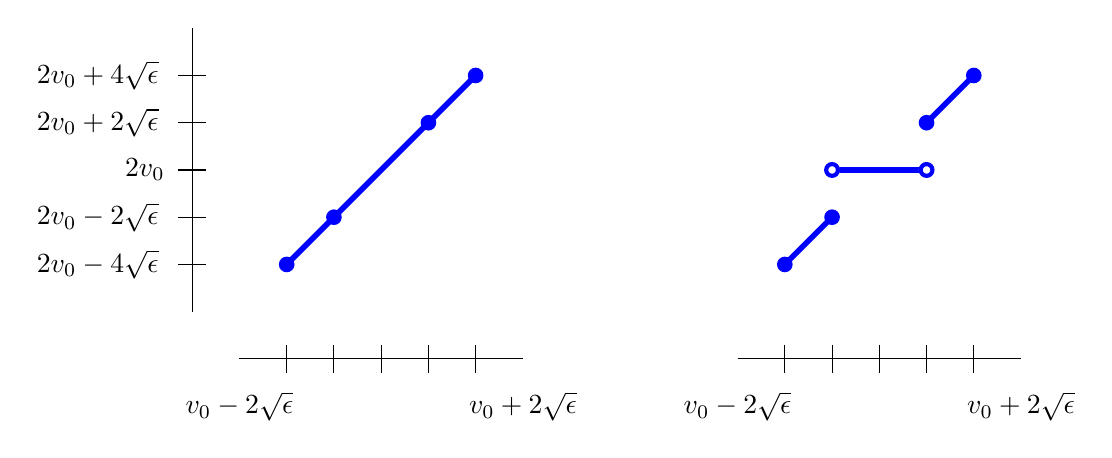
\begin{tikzpicture}[scale=.6]

\node at (0,-1) {$v_0-2\sqrt{\eps}$};
\node at (6,-1) {$v_0 + 2\sqrt{\eps}$};

\draw (0,0) -- (6,0);
\draw (1,-.3) -- (1,.3);
\draw (2,-.3) -- (2,.3);
\draw (3,-.3) -- (3,.3);
\draw (4,-.3) -- (4,.3);
\draw (5,-.3) -- (5,.3);

\draw[line width=2, blue] (1,2)--(5,6);
\node[circle,fill,inner sep=2pt, blue] at (1,2) {};
\node[circle,fill,inner sep=2pt, blue] at (2,3) {};
\node[circle,fill,inner sep=2pt, blue] at (4,5) {};
\node[circle,fill,inner sep=2pt, blue] at (5,6) {};

\draw (-1,1)--(-1,7);
\draw (-1.3,3)--(-0.7,3);
\draw (-1.3,2)--(-0.7,2);
\draw (-1.3,4)--(-0.7,4);
\draw (-1.3,5)--(-0.7,5);
\draw (-1.3,6)--(-0.7,6);

\node at (-3,3) {$2v_0-2\sqrt{\eps}$};
\node at (-3,2) {$2v_0-4\sqrt{\epsilon}$};
\node at (-2,4) {$2v_0$};
\node at (-3,6) {$2v_0+4\sqrt{\epsilon}$};
\node at (-3,5) {$2v_0+2\sqrt{\eps}$};


\begin{scope}[xshift=300]
\node at (0,-1) {$v_0-2\sqrt{\eps}$};
\node at (6,-1) {$v_0 + 2\sqrt{\epsilon}$};

\draw (0,0) -- (6,0);
\draw (1,-.3) -- (1,.3);
\draw (2,-.3) -- (2,.3);
\draw (3,-.3) -- (3,.3);
\draw (4,-.3) -- (4,.3);
\draw (5,-.3) -- (5,.3);

\draw[line width=2, blue] (1,2)--(2,3);
\draw[line width=2, blue] (2,4)--(4,4);
\draw[line width=2, blue] (4,5)--(5,6);
\node[circle,fill,inner sep=2pt, blue] at (1,2) {};
\node[circle,fill,inner sep=2pt, blue] at (2,3) {};
\node[circle,fill,inner sep=2pt, white] at (2,4) {};
\node[circle, draw, inner sep=1.5pt, line width=1.5,blue] at (2,4) {};
\node[circle,fill,inner sep=2pt, white] at (4,4) {};
\node[circle, draw, inner sep=1.5pt, line width=1.5,blue] at (4,4) {};
\node[circle,fill,inner sep=2pt, blue] at (4,5) {};
\node[circle,fill,inner sep=2pt, blue] at (5,6) {};


\end{scope}

\end{tikzpicture}

\end{document}